
\chapter{QUADRO METODOLÓGICO}
\par O quadro metodológico é a descrição dos passos realizados para a 
execução do projeto. Serão listados, nos tópicos a seguir, os itens essenciais
no desenvolvimento do trabalho, sendo eles as técnicas, procedimentos, práticas e instrumentos
utilizados, o contexto de aplicação, os participantes, o orçamento, o cronograma
e o tipo de pesquisa utilizado.

\section{Tipo de pesquisa}

\par Para \citeonline[p.42]{pesquisa_social_gil}, a pesquisa tem um caráter
pragmático, é um “processo formal e sistemático de desenvolvimento do método científico. 
O objetivo fundamental da pesquisa é descobrir respostas para problemas mediante
o emprego de procedimentos científicos”.
\par Este projeto terá como base a metodologia de pesquisa aplicada, pois
será desenvolvida uma aplicação inteligente utilizando Algoritmos Genéticos para
o auxílio na tomada de decisão sobre a produção de calças de uma confecção.

\par \citeonline[p.35]{livro_metodos_de_pesquisa} afirmam que o método de
pesquisa aplicada, "objetiva gerar conhecimentos para aplicação prática, dirigidos a
solução de problemas específicos. Envolve verdades e interesses locais."  

\par Segundo \citeonline{livro_metodologia_de_estudo_de_pesquisa}, a pesquisa
aplicada tem como motivação básica a solução de problemas
concretos, práticos e operacionais e também pode ser chamada de pesquisa
empírica pois o pesquisador precisa ir a campo, conversar com pessoas e
presenciar relações sociais.

\section{Contexto de pesquisa}

\par Sabe-se que com a alta competitividade no mercado, empresas cada vez mais
buscam diferenciais competitivos para seus produtos e, neste cenário, a ideia
de redução de custos se torna essencial uma vez que tal redução pode ser
refletida no preço dos produtos permitindo que estes se diferenciem. Dentre
os fatores que viabilizam tais reduções está a otimização de processos que
consistem em organizar os procedimentos relacionados à produção de forma que
estes se tornem mais eficazes.

\par O software desenvolvido neste trabalho visa organizar uma linha de produção
de forma que esta se torne o mais eficiente possível. Será utilizada como
base uma determinada fábrica de confecção de calças situada na cidade de
Cachoeira de Minas - MG, porém a base de conhecimento pode ser aplicada a outros
tipos de negócios que seguem o mesmo padrão de desenvolvimento de produtos.


\section{Participantes}

\par Jonathan Ribeiro dos Santos, acadêmico do 7o período do curso de Bacharelado em
Sistemas de Informação pela Universidade do Vale do Sapucaí. Possui
conhecimentos em HTML, CSS, Java Script, PHP, C, Java, PostgreSQL, redes
estruturadas e Microsoft Windows Server e atuará como desenvolvedor desse
projeto.

\par Sandro Augusto de Oliveira, acadêmico do 7o período do curso de Bacharelado
em Sistemas de Informação pela Universidade do Vale do Sapucaí. Possui
conhecimentos em HTML, CSS, Java Script, PHP, C, Java, PostgreSQL, MySQL, redes
estruturadas e Microsoft Windows Server e sistema operacional Linux e atuará
como desenvolvedor desse projeto.

\par Prof. Roberto Ribeiro Rocha, graduado em Ciência da Computação pela
faculdade de Administração e Informática – FAI (2002), possui especialização
em Produção de Software Livre pela Universidade Federal de Lavras – UFLA (2006)
e mestrado em Ciência e Tecnologia da Informação na Universidade Federal de Itajubá – UNIFEI (2013).
Foi analista de sistemas na Liveware Tecnologia a Serviço Ltda e integrante da equipe de TI na Megatron
Fios e Cabos Especiais. Possui experiência na área de ciência da computação, com ênfase em arquitetura de
sistemas de computação, software livre e Linux. Atualmente é professor no curso de Sistemas de Informação 
na Univás e atuará como orientador neste projeto.

% \par Propietário da fábrica de tecidos, atuará como fornecedor de requisitos
% para o projeto.

\par O trabalho de documentação e desenvolvimento será realizado em conjunto por
Sandro e Jonathan com a orientação do professor Roberto. O Gestor da empresa
será o ponto de contato em caso de dúvidas quanto ao processo de produção da
fábrica.

\section{Instrumentos}

\par Segundo \citeonline{aula_joelma_26_03_15}, instrumentos de pesquisa são a
forma que os dados serão coletados para a realização do trabalho, podendo ser,
dentre outras formas, por meio de reuniões, questionários e entrevistas. Para
este projeto utilizaremos os instrumentos descritos nas subsessões a seguir.

\subsection{Entrevistas}
\par Segundo \citeonline{metodoliga_qualitativas_na_sociologia}, entrevista é
uma interação entre duas pessoas em que uma representa o entrevistador, 
que através de perguntas, obtêm informações por parte de outra pessoa que
representa o entrevistado.


% entrevista é um
% “processo de interação social entre duas pessoas na qual uma delas, o entrevistador,
% tem por objetivo a obtenção de informações por parte do outro, o entrevistado”



\par Será realizada uma entrevista com o dono da empresa de confecção com o
objetivo de entender seu modelo de negócio para que então seja possível começar
a fazer o levantamento dos requisitos do sistema. Para
\citeonline[p.128]{pressman2011engenharia}, levantamento de requisitos de
software consiste em

\begin{citacao}
perguntar ao cliente, aos usuários e aos demais interessados quais são os
objetivos para o sistema ou produto, o que deve ser alcançado, como o sistema ou
produto atenda às necessidades da empresa e, por fim, como o sistema ou produto
deve ser utilizado no dia a dia.
\end{citacao} 


\subsection{Reuniões}
\par De acordo com \citeonline{ref_reuniao}, reunião é o ajuntamento de
pessoas para se tratar de um determinado assunto em que é necessário que se
tenha conclusões sobre as questões que foram discutidas.

\par Durante o desenvolvimento do projeto poderão ser realizadas reuniões
com o proprietário da fábrica de calças para saneamento de dúvidas, sugestões e
outros assuntos que possam surgir.

\section{Procedimentos}

\par Esta sessão descreve os procedimentos a serem realizados na execução do
projeto.

 \begin{itemize}

	\item Fazer uma prova de conceito com algoritmos genéticos para eliminar
	dúvidas cruciais sobre a viabilidade do projeto;
	  
	\item Realizar a coleta dos requisitos com o gestor da empresa;
	\par Descrever sobre os requisitos
	
	\item Executar procedimentos referente à engenharia do software;
	
	\subsection{Realzação da Modelagem da base de dados};
	
	
	\item Codificar o projeto;
	 Problemas encontrados no desenvolvimento

	\item Realizar testes.
	 
 \end{itemize}
 
 \par Realizando todos os passos descritos acima, teremos como resultado final o
 projeto finalizado.

\newpage

\section{Cronograma}

\par Abaixo o cronograma de desenvolvimento do projeto.

\begin{table}[ht!]
\centering
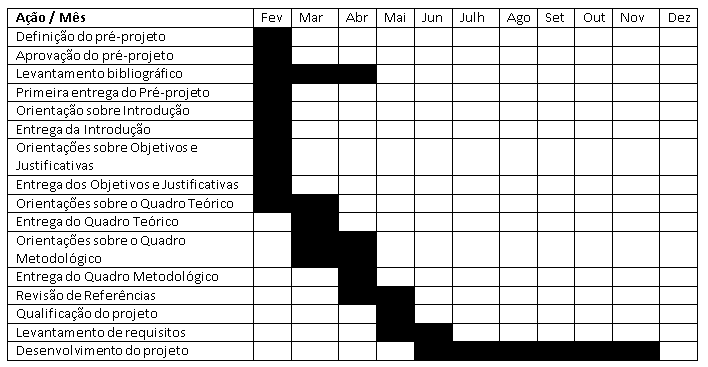
\includegraphics[width=150mm]{./imagens/tabela.jpg}
\caption{Cronograma de desenvolvimento do projeto. \textbf{Fonte:} Desenvolvido
pelos autores.}
\end{table}
\newpage

\section{Orçamento}

\par Os gastos previstos até o momento serão os de impressão, energia, combustível e um
curso de apresentação de projetos que estamos planejando fazer no SENAC. No
total, o custo será de cerca de 400 reais. 

% \label{cap:quadroMetodologico}
% 
% \par Conteúdo do quadro metodológico. Perceba a forma que se coloca uma palavra entre aspas: o \LaTeX~oferece muita ``facilitade de formatação''.
% 
% Exemplo de código Java:
% 
% \begin{lstlisting} [style=custom_Java,caption={[Métodos da classe \texttt{FilmeBean}]{Métodos da classe \texttt{FilmeBean}. \textbf{Fonte:} Elaborado pelos autores.}}, label=fig:metodosclassebean] 	
% 	public FilmeBean(){  
%        //...
%    	}	
%    	
% 	public void saveMovie(){
% 		setListActorSelected();		
% 		if(this.movieDAO.saveMovieGraph(this.movieTo)){
% 			FacesContext.getCurrentInstance().addMessage(null, 
% 			   new FacesMessage("Filme cadastrado com sucesso!")); 
% 		}else{
% 			//...
% 		}		
% 		this.limpaCampos();
% 	}
% \end{lstlisting}
% 
% \par Agora será mostrado o exemplo do uso de fluxo de eventos apresentado no Quadro~\ref{quad:fluxo_evento_cadastro_filme}.
% 
% \begin{quadro}[h!]
%   \begin{fluxoDeEventos}
  \addTitle{Cadastrar filme}
  \addrow{Ator principal}{Administrador}
  %\addrow{Ator secundário}{Sistema de cartão}
  \addrow{Pré-requisitos}{Estar logado no sistema}

  \startBasicFlow{Ator} {Sistema}
  \addItemOne{Seleciona menu cadastro}
  \addItemOne{Clica na opção cadastrar filme}
  \addItemTwo{Abre interface de cadastro de filme}
  \addItemOne{Preenche formulário}
  \addItemOne{Clica no botão salvar}
  \addItemTwo{Salva e informa sucesso no cadastro}

  \startAlternativeFlow{Fluxo alternativo 1}
  \addItemOne{No item 5, formulário não preenchido}
  \addItemTwo{Exibe mensagem de necessidade de preenchimento de formulário}

  \startAlternativeFlow{Fluxo alternativo 2}
  \addItemOne{No item 6, inserido filme já cadastrado}
  \addItemTwo{Informa mensagem de filme já cadastrado}
\end{fluxoDeEventos}

%   \caption[Fluxo de eventos para cadastro de filme]
%            {Fluxo de eventos para cadastro de filme. \textbf{Fonte:} Elaborado pelos autores}
%   \label{quad:fluxo_evento_cadastro_filme}
% \end{quadro}
% 
% \par Outro exemplo é ilustrado na Figura~\ref{fig:bluesky}. Neste caso um código XML foi embutido dentro de um ambiente de figura, para que este código seja incluído no índice de figuras adequadamente.
%  
% \begin{figure}[ht!]
%   \begin{lstlisting} [style=custom_XML]
% 	...
% 	<context-param>
% 		<param-name>primefaces.THEME<\param-name>
% 		<param-value>bluesky<\param-value>
% 	<\context-param>
% 	...
%   \end{lstlisting}
%   \caption[Incluindo o tema \textit{BlueSky} ao contexto do projeto]
%           {Incluíndo o tema \textit{BlueSky} ao contexto do projeto. \textbf{Fonte:} Elaborado pelos autores.}
%   \label{fig:bluesky}
% \end{figure}
